\documentclass[1p]{elsarticle_modified}
%\bibliographystyle{elsarticle-num}

%\usepackage[colorlinks]{hyperref}
%\usepackage{abbrmath_seonhwa} %\Abb, \Ascr, \Acal ,\Abf, \Afrak
\usepackage{amsfonts}
\usepackage{amssymb}
\usepackage{amsmath}
\usepackage{amsthm}
\usepackage{scalefnt}
\usepackage{amsbsy}
\usepackage{kotex}
\usepackage{caption}
\usepackage{subfig}
\usepackage{color}
\usepackage{graphicx}
\usepackage{xcolor} %% white, black, red, green, blue, cyan, magenta, yellow
\usepackage{float}
\usepackage{setspace}
\usepackage{hyperref}

\usepackage{tikz}
\usetikzlibrary{arrows}

\usepackage{multirow}
\usepackage{array} % fixed length table
\usepackage{hhline}

%%%%%%%%%%%%%%%%%%%%%
\makeatletter
\renewcommand*\env@matrix[1][\arraystretch]{%
	\edef\arraystretch{#1}%
	\hskip -\arraycolsep
	\let\@ifnextchar\new@ifnextchar
	\array{*\c@MaxMatrixCols c}}
\makeatother %https://tex.stackexchange.com/questions/14071/how-can-i-increase-the-line-spacing-in-a-matrix
%%%%%%%%%%%%%%%

\usepackage[normalem]{ulem}

\newcommand{\msout}[1]{\ifmmode\text{\sout{\ensuremath{#1}}}\else\sout{#1}\fi}
%SOURCE: \msout is \stkout macro in https://tex.stackexchange.com/questions/20609/strikeout-in-math-mode

\newcommand{\cancel}[1]{
	\ifmmode
	{\color{red}\msout{#1}}
	\else
	{\color{red}\sout{#1}}
	\fi
}

\newcommand{\add}[1]{
	{\color{blue}\uwave{#1}}
}

\newcommand{\replace}[2]{
	\ifmmode
	{\color{red}\msout{#1}}{\color{blue}\uwave{#2}}
	\else
	{\color{red}\sout{#1}}{\color{blue}\uwave{#2}}
	\fi
}

\newcommand{\Sol}{\mathcal{S}} %segment
\newcommand{\D}{D} %diagram
\newcommand{\A}{\mathcal{A}} %arc


%%%%%%%%%%%%%%%%%%%%%%%%%%%%%5 test

\def\sl{\operatorname{\textup{SL}}(2,\Cbb)}
\def\psl{\operatorname{\textup{PSL}}(2,\Cbb)}
\def\quan{\mkern 1mu \triangleright \mkern 1mu}

\theoremstyle{definition}
\newtheorem{thm}{Theorem}[section]
\newtheorem{prop}[thm]{Proposition}
\newtheorem{lem}[thm]{Lemma}
\newtheorem{ques}[thm]{Question}
\newtheorem{cor}[thm]{Corollary}
\newtheorem{defn}[thm]{Definition}
\newtheorem{exam}[thm]{Example}
\newtheorem{rmk}[thm]{Remark}
\newtheorem{alg}[thm]{Algorithm}

\newcommand{\I}{\sqrt{-1}}
\begin{document}

%\begin{frontmatter}
%
%\title{Boundary parabolic representations of knots up to 8 crossings}
%
%%% Group authors per affiliation:
%\author{Yunhi Cho} 
%\address{Department of Mathematics, University of Seoul, Seoul, Korea}
%\ead{yhcho@uos.ac.kr}
%
%
%\author{Seonhwa Kim} %\fnref{s_kim}}
%\address{Center for Geometry and Physics, Institute for Basic Science, Pohang, 37673, Korea}
%\ead{ryeona17@ibs.re.kr}
%
%\author{Hyuk Kim}
%\address{Department of Mathematical Sciences, Seoul National University, Seoul 08826, Korea}
%\ead{hyukkim@snu.ac.kr}
%
%\author{Seokbeom Yoon}
%\address{Department of Mathematical Sciences, Seoul National University, Seoul, 08826,  Korea}
%\ead{sbyoon15@snu.ac.kr}
%
%\begin{abstract}
%We find all boundary parabolic representation of knots up to 8 crossings.
%
%\end{abstract}
%\begin{keyword}
%    \MSC[2010] 57M25 
%\end{keyword}
%
%\end{frontmatter}

%\linenumbers
%\tableofcontents
%
\newcommand\colored[1]{\textcolor{white}{\rule[-0.35ex]{0.8em}{1.4ex}}\kern-0.8em\color{red} #1}%
%\newcommand\colored[1]{\textcolor{white}{ #1}\kern-2.17ex	\textcolor{white}{ #1}\kern-1.81ex	\textcolor{white}{ #1}\kern-2.15ex\color{red}#1	}

{\Large $\underline{12a_{1212}~(K12a_{1212})}$}

\setlength{\tabcolsep}{10pt}
\renewcommand{\arraystretch}{1.6}
\vspace{1cm}\begin{tabular}{m{100pt}>{\centering\arraybackslash}m{274pt}}
\multirow{5}{120pt}{
	\centering
	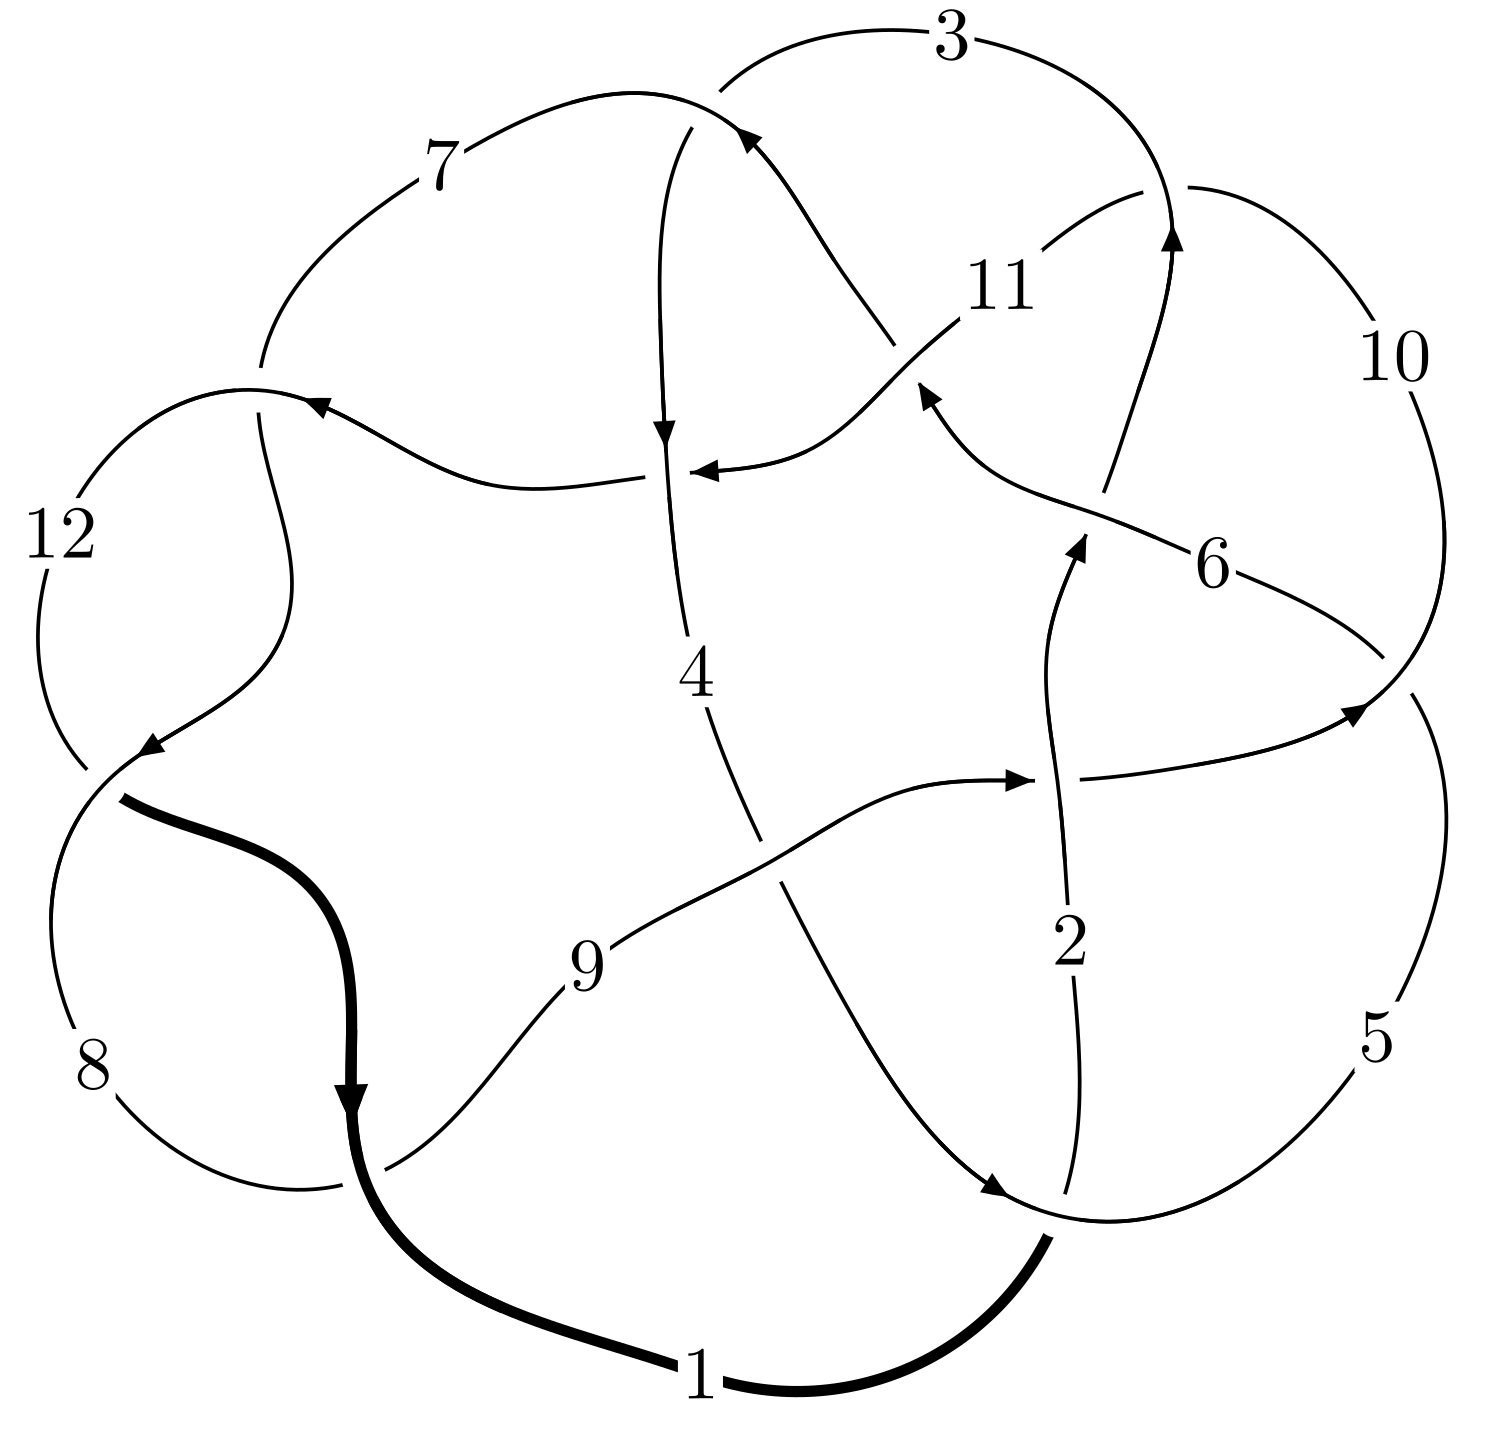
\includegraphics[width=112pt]{../../../GIT/diagram.site/Diagrams/png/2013_12a_1212.png}\\
\ \ \ A knot diagram\footnotemark}&
\allowdisplaybreaks
\textbf{Linearized knot diagam} \\
\cline{2-2}
 &
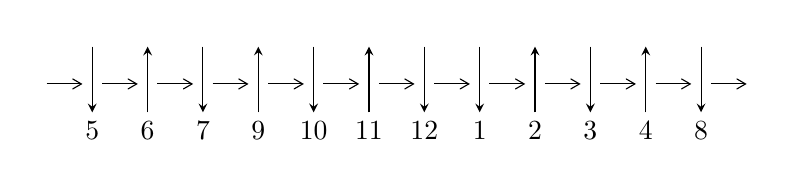
\begin{tikzpicture}[x=20pt, y=17pt]
	% nodes
	\node (C0) at (0, 0) {};
	\node (C1) at (1, 0) {};
	\node (C1U) at (1, +1) {};
	\node (C1D) at (1, -1) {5};

	\node (C2) at (2, 0) {};
	\node (C2U) at (2, +1) {};
	\node (C2D) at (2, -1) {6};

	\node (C3) at (3, 0) {};
	\node (C3U) at (3, +1) {};
	\node (C3D) at (3, -1) {7};

	\node (C4) at (4, 0) {};
	\node (C4U) at (4, +1) {};
	\node (C4D) at (4, -1) {9};

	\node (C5) at (5, 0) {};
	\node (C5U) at (5, +1) {};
	\node (C5D) at (5, -1) {10};

	\node (C6) at (6, 0) {};
	\node (C6U) at (6, +1) {};
	\node (C6D) at (6, -1) {11};

	\node (C7) at (7, 0) {};
	\node (C7U) at (7, +1) {};
	\node (C7D) at (7, -1) {12};

	\node (C8) at (8, 0) {};
	\node (C8U) at (8, +1) {};
	\node (C8D) at (8, -1) {1};

	\node (C9) at (9, 0) {};
	\node (C9U) at (9, +1) {};
	\node (C9D) at (9, -1) {2};

	\node (C10) at (10, 0) {};
	\node (C10U) at (10, +1) {};
	\node (C10D) at (10, -1) {3};

	\node (C11) at (11, 0) {};
	\node (C11U) at (11, +1) {};
	\node (C11D) at (11, -1) {4};

	\node (C12) at (12, 0) {};
	\node (C12U) at (12, +1) {};
	\node (C12D) at (12, -1) {8};
	\node (C13) at (13, 0) {};

	% arrows
	\draw[->,>={angle 60}]
	(C0) edge (C1) (C1) edge (C2) (C2) edge (C3) (C3) edge (C4) (C4) edge (C5) (C5) edge (C6) (C6) edge (C7) (C7) edge (C8) (C8) edge (C9) (C9) edge (C10) (C10) edge (C11) (C11) edge (C12) (C12) edge (C13) ;	\draw[->,>=stealth]
	(C1U) edge (C1D) (C2D) edge (C2U) (C3U) edge (C3D) (C4D) edge (C4U) (C5U) edge (C5D) (C6D) edge (C6U) (C7U) edge (C7D) (C8U) edge (C8D) (C9D) edge (C9U) (C10U) edge (C10D) (C11D) edge (C11U) (C12U) edge (C12D) ;
	\end{tikzpicture} \\
\hhline{~~} \\& 
\textbf{Solving Sequence} \\ \cline{2-2} 
 &
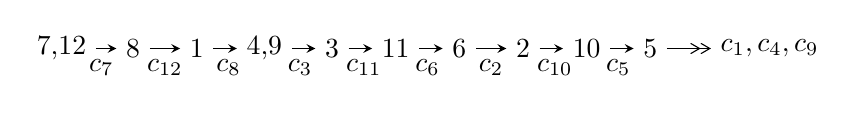
\begin{tikzpicture}[x=23pt, y=7pt]
	% node
	\node (A0) at (-1/8, 0) {7,12};
	\node (A1) at (1, 0) {8};
	\node (A2) at (2, 0) {1};
	\node (A3) at (49/16, 0) {4,9};
	\node (A4) at (33/8, 0) {3};
	\node (A5) at (41/8, 0) {11};
	\node (A6) at (49/8, 0) {6};
	\node (A7) at (57/8, 0) {2};
	\node (A8) at (65/8, 0) {10};
	\node (A9) at (73/8, 0) {5};
	\node (C1) at (1/2, -1) {$c_{7}$};
	\node (C2) at (3/2, -1) {$c_{12}$};
	\node (C3) at (5/2, -1) {$c_{8}$};
	\node (C4) at (29/8, -1) {$c_{3}$};
	\node (C5) at (37/8, -1) {$c_{11}$};
	\node (C6) at (45/8, -1) {$c_{6}$};
	\node (C7) at (53/8, -1) {$c_{2}$};
	\node (C8) at (61/8, -1) {$c_{10}$};
	\node (C9) at (69/8, -1) {$c_{5}$};
	\node (A10) at (11, 0) {$c_{1},c_{4},c_{9}$};

	% edge
	\draw[->,>=stealth]	
	(A0) edge (A1) (A1) edge (A2) (A2) edge (A3) (A3) edge (A4) (A4) edge (A5) (A5) edge (A6) (A6) edge (A7) (A7) edge (A8) (A8) edge (A9) ;
	\draw[->>,>={angle 60}]	
	(A9) edge (A10);
\end{tikzpicture} \\ 

\end{tabular} \\

\footnotetext{
The image of knot diagram is generated by the software ``\textbf{Draw programme}" developed by Andrew Bartholomew(\url{http://www.layer8.co.uk/maths/draw/index.htm\#Running-draw}), where we modified some parts for our purpose(\url{https://github.com/CATsTAILs/LinksPainter}).
}\phantom \\ \newline 
\centering \textbf{Ideals for irreducible components\footnotemark of $X_{\text{par}}$} 
 
\begin{align*}
I^u_{1}&=\langle 
-8237647 u^{24}-46666064 u^{23}+\cdots+1517168 b-99699472,\\
\phantom{I^u_{1}}&\phantom{= \langle  }50602827 u^{24}+326501622 u^{23}+\cdots+3034336 a+1024079008,\;u^{25}+8 u^{24}+\cdots-32 u+32\rangle \\
I^u_{2}&=\langle 
91 u^{12}-255 u^{11}+\cdots+82 b+126,\;68 u^{12}-191 u^{11}+\cdots+164 a+1075,\\
\phantom{I^u_{2}}&\phantom{= \langle  }u^{13}-4 u^{12}- u^{11}+24 u^{10}-21 u^9-44 u^8+60 u^7+23 u^6-37 u^5-10 u^4-15 u^3+24 u^2+3 u-1\rangle \\
I^u_{3}&=\langle 
- u^{51} a-375 u^{51}+\cdots+a+909,\;316 u^{51} a-805 u^{51}+\cdots+2748 a-4408,\;u^{52}-6 u^{51}+\cdots+18 u+1\rangle \\
I^u_{4}&=\langle 
b+1,\;a,\;u-1\rangle \\
\\
\end{align*}
\raggedright * 4 irreducible components of $\dim_{\mathbb{C}}=0$, with total 143 representations.\\
\footnotetext{All coefficients of polynomials are rational numbers. But the coefficients are sometimes approximated in decimal forms when there is not enough margin.}
\newpage
\renewcommand{\arraystretch}{1}
\centering \section*{I. $I^u_{1}= \langle -8.24\times10^{6} u^{24}-4.67\times10^{7} u^{23}+\cdots+1.52\times10^{6} b-9.97\times10^{7},\;5.06\times10^{7} u^{24}+3.27\times10^{8} u^{23}+\cdots+3.03\times10^{6} a+1.02\times10^{9},\;u^{25}+8 u^{24}+\cdots-32 u+32 \rangle$}
\flushleft \textbf{(i) Arc colorings}\\
\begin{tabular}{m{7pt} m{180pt} m{7pt} m{180pt} }
\flushright $a_{7}=$&$\begin{pmatrix}1\\0\end{pmatrix}$ \\
\flushright $a_{12}=$&$\begin{pmatrix}0\\u\end{pmatrix}$ \\
\flushright $a_{8}=$&$\begin{pmatrix}1\\u^2\end{pmatrix}$ \\
\flushright $a_{1}=$&$\begin{pmatrix}- u\\- u^3+u\end{pmatrix}$ \\
\flushright $a_{4}=$&$\begin{pmatrix}-16.6767 u^{24}-107.602 u^{23}+\cdots+549.463 u-337.497\\5.42962 u^{24}+30.7587 u^{23}+\cdots-86.2463 u+65.7142\end{pmatrix}$ \\
\flushright $a_{9}=$&$\begin{pmatrix}- u^2+1\\- u^4+2 u^2\end{pmatrix}$ \\
\flushright $a_{3}=$&$\begin{pmatrix}-11.2471 u^{24}-76.8437 u^{23}+\cdots+463.217 u-271.783\\5.42962 u^{24}+30.7587 u^{23}+\cdots-86.2463 u+65.7142\end{pmatrix}$ \\
\flushright $a_{11}=$&$\begin{pmatrix}14.2117 u^{24}+90.2914 u^{23}+\cdots-434.374 u+271.092\\3.50175 u^{24}+25.1620 u^{23}+\cdots-177.375 u+100.690\end{pmatrix}$ \\
\flushright $a_{6}=$&$\begin{pmatrix}11.8969 u^{24}+71.8441 u^{23}+\cdots-240.897 u+176.461\\23.6941 u^{24}+153.970 u^{23}+\cdots-804.871 u+491.973\end{pmatrix}$ \\
\flushright $a_{2}=$&$\begin{pmatrix}-6.67636 u^{24}-39.5426 u^{23}+\cdots+111.025 u-87.1118\\-17.0962 u^{24}-108.869 u^{23}+\cdots+532.397 u-332.532\end{pmatrix}$ \\
\flushright $a_{10}=$&$\begin{pmatrix}-3.98808 u^{24}-18.4219 u^{23}+\cdots-69.4800 u+9.06809\\-19.3622 u^{24}-117.721 u^{23}+\cdots+440.516 u-303.830\end{pmatrix}$ \\
\flushright $a_{5}=$&$\begin{pmatrix}15.1868 u^{24}+104.234 u^{23}+\cdots-656.947 u+380.440\\1.94010 u^{24}+24.7858 u^{23}+\cdots-406.617 u+192.420\end{pmatrix}$\\&\end{tabular}
\flushleft \textbf{(ii) Obstruction class $= -1$}\\~\\
\flushleft \textbf{(iii) Cusp Shapes $= -\frac{5240957}{94823} u^{24}-\frac{67769311}{189646} u^{23}+\cdots+\frac{187802884}{94823} u-\frac{111850042}{94823}$}\\~\\
\newpage\renewcommand{\arraystretch}{1}
\flushleft \textbf{(iv) u-Polynomials at the component}\newline \\
\begin{tabular}{m{50pt}|m{274pt}}
Crossings & \hspace{64pt}u-Polynomials at each crossing \\
\hline $$\begin{aligned}c_{1},c_{3}\end{aligned}$$&$\begin{aligned}
&u^{25}- u^{24}+\cdots-5 u+1
\end{aligned}$\\
\hline $$\begin{aligned}c_{2}\end{aligned}$$&$\begin{aligned}
&u^{25}-16 u^{24}+\cdots+7168 u-1024
\end{aligned}$\\
\hline $$\begin{aligned}c_{4},c_{11}\end{aligned}$$&$\begin{aligned}
&u^{25}+7 u^{24}+\cdots+10 u+2
\end{aligned}$\\
\hline $$\begin{aligned}c_{5},c_{10}\end{aligned}$$&$\begin{aligned}
&u^{25}+4 u^{24}+\cdots-3 u+1
\end{aligned}$\\
\hline $$\begin{aligned}c_{6},c_{9}\end{aligned}$$&$\begin{aligned}
&u^{25}+2 u^{24}+\cdots+7 u-1
\end{aligned}$\\
\hline $$\begin{aligned}c_{7},c_{8},c_{12}\end{aligned}$$&$\begin{aligned}
&u^{25}-8 u^{24}+\cdots-32 u-32
\end{aligned}$\\
\hline
\end{tabular}\\~\\
\newpage\renewcommand{\arraystretch}{1}
\flushleft \textbf{(v) Riley Polynomials at the component}\newline \\
\begin{tabular}{m{50pt}|m{274pt}}
Crossings & \hspace{64pt}Riley Polynomials at each crossing \\
\hline $$\begin{aligned}c_{1},c_{3}\end{aligned}$$&$\begin{aligned}
&y^{25}-7 y^{24}+\cdots+25 y-1
\end{aligned}$\\
\hline $$\begin{aligned}c_{2}\end{aligned}$$&$\begin{aligned}
&y^{25}+18 y^{23}+\cdots-11010048 y-1048576
\end{aligned}$\\
\hline $$\begin{aligned}c_{4},c_{11}\end{aligned}$$&$\begin{aligned}
&y^{25}-21 y^{24}+\cdots-100 y-4
\end{aligned}$\\
\hline $$\begin{aligned}c_{5},c_{10}\end{aligned}$$&$\begin{aligned}
&y^{25}-32 y^{24}+\cdots-3 y-1
\end{aligned}$\\
\hline $$\begin{aligned}c_{6},c_{9}\end{aligned}$$&$\begin{aligned}
&y^{25}-2 y^{24}+\cdots+15 y-1
\end{aligned}$\\
\hline $$\begin{aligned}c_{7},c_{8},c_{12}\end{aligned}$$&$\begin{aligned}
&y^{25}-24 y^{24}+\cdots-6656 y-1024
\end{aligned}$\\
\hline
\end{tabular}\\~\\
\newpage\flushleft \textbf{(vi) Complex Volumes and Cusp Shapes}
$$\begin{array}{c|c|c}  
\text{Solutions to }I^u_{1}& \I (\text{vol} + \sqrt{-1}CS) & \text{Cusp shape}\\
 \hline 
\begin{aligned}
u &= \phantom{-}0.724396 + 0.814795 I \\
a &= -0.033461 + 1.260570 I \\
b &= -1.18344 - 0.87037 I\end{aligned}
 & -0.1080 - 15.3508 I & -2.78225 + 10.65242 I \\ \hline\begin{aligned}
u &= \phantom{-}0.724396 - 0.814795 I \\
a &= -0.033461 - 1.260570 I \\
b &= -1.18344 + 0.87037 I\end{aligned}
 & -0.1080 + 15.3508 I & -2.78225 - 10.65242 I \\ \hline\begin{aligned}
u &= \phantom{-}0.317167 + 1.050900 I \\
a &= \phantom{-}0.616196 - 0.409967 I \\
b &= -0.827326 + 0.814013 I\end{aligned}
 & \phantom{-}1.10917 + 9.40524 I & \phantom{-}0.04392 - 9.75471 I \\ \hline\begin{aligned}
u &= \phantom{-}0.317167 - 1.050900 I \\
a &= \phantom{-}0.616196 + 0.409967 I \\
b &= -0.827326 - 0.814013 I\end{aligned}
 & \phantom{-}1.10917 - 9.40524 I & \phantom{-}0.04392 + 9.75471 I \\ \hline\begin{aligned}
u &= \phantom{-}0.664502 + 0.907721 I \\
a &= -0.137319 - 0.952600 I \\
b &= \phantom{-}1.034870 + 0.744773 I\end{aligned}
 & -2.89814 - 6.85193 I & -7.15013 + 8.59668 I \\ \hline\begin{aligned}
u &= \phantom{-}0.664502 - 0.907721 I \\
a &= -0.137319 + 0.952600 I \\
b &= \phantom{-}1.034870 - 0.744773 I\end{aligned}
 & -2.89814 + 6.85193 I & -7.15013 - 8.59668 I \\ \hline\begin{aligned}
u &= \phantom{-}1.20846\phantom{ +0.000000I} \\
a &= \phantom{-}1.27084\phantom{ +0.000000I} \\
b &= \phantom{-}1.16050\phantom{ +0.000000I}\end{aligned}
 & \phantom{-}0.266082\phantom{ +0.000000I} & -11.4730\phantom{ +0.000000I} \\ \hline\begin{aligned}
u &= -1.266140 + 0.080450 I \\
a &= -0.243476 - 0.336575 I \\
b &= \phantom{-}0.274129 + 1.260920 I\end{aligned}
 & -0.76316 + 4.31765 I & -0.89966 - 6.91445 I \\ \hline\begin{aligned}
u &= -1.266140 - 0.080450 I \\
a &= -0.243476 + 0.336575 I \\
b &= \phantom{-}0.274129 - 1.260920 I\end{aligned}
 & -0.76316 - 4.31765 I & -0.89966 + 6.91445 I \\ \hline\begin{aligned}
u &= \phantom{-}0.692428\phantom{ +0.000000I} \\
a &= \phantom{-}4.42334\phantom{ +0.000000I} \\
b &= \phantom{-}0.311066\phantom{ +0.000000I}\end{aligned}
 & \phantom{-}0.704588\phantom{ +0.000000I} & -85.9750\phantom{ +0.000000I}\\
 \hline 
 \end{array}$$\newpage$$\begin{array}{c|c|c}  
\text{Solutions to }I^u_{1}& \I (\text{vol} + \sqrt{-1}CS) & \text{Cusp shape}\\
 \hline 
\begin{aligned}
u &= -1.379800 + 0.232274 I \\
a &= -0.202915 - 0.655047 I \\
b &= -0.97116 + 1.06639 I\end{aligned}
 & -5.14325 + 3.90529 I & \phantom{-}0.85581 - 4.51378 I \\ \hline\begin{aligned}
u &= -1.379800 - 0.232274 I \\
a &= -0.202915 + 0.655047 I \\
b &= -0.97116 - 1.06639 I\end{aligned}
 & -5.14325 - 3.90529 I & \phantom{-}0.85581 + 4.51378 I \\ \hline\begin{aligned}
u &= \phantom{-}0.068901 + 0.526930 I \\
a &= -0.19999 + 1.73646 I \\
b &= \phantom{-}0.622226 - 0.843745 I\end{aligned}
 & \phantom{-}3.21655 - 2.10472 I & \phantom{-}4.13419 + 3.80054 I \\ \hline\begin{aligned}
u &= \phantom{-}0.068901 - 0.526930 I \\
a &= -0.19999 - 1.73646 I \\
b &= \phantom{-}0.622226 + 0.843745 I\end{aligned}
 & \phantom{-}3.21655 + 2.10472 I & \phantom{-}4.13419 - 3.80054 I \\ \hline\begin{aligned}
u &= \phantom{-}0.213598 + 0.439117 I \\
a &= \phantom{-}0.933169 + 0.905622 I \\
b &= -0.321753 - 0.450048 I\end{aligned}
 & -0.214830 - 1.179340 I & -2.40251 + 6.38928 I \\ \hline\begin{aligned}
u &= \phantom{-}0.213598 - 0.439117 I \\
a &= \phantom{-}0.933169 - 0.905622 I \\
b &= -0.321753 + 0.450048 I\end{aligned}
 & -0.214830 + 1.179340 I & -2.40251 - 6.38928 I \\ \hline\begin{aligned}
u &= -1.59465 + 0.30004 I \\
a &= \phantom{-}0.522691 + 0.816481 I \\
b &= \phantom{-}1.39230 - 0.76184 I\end{aligned}
 & -10.2598 + 11.2873 I & -9.23051 - 7.41391 I \\ \hline\begin{aligned}
u &= -1.59465 - 0.30004 I \\
a &= \phantom{-}0.522691 - 0.816481 I \\
b &= \phantom{-}1.39230 + 0.76184 I\end{aligned}
 & -10.2598 - 11.2873 I & -9.23051 + 7.41391 I \\ \hline\begin{aligned}
u &= -1.61150 + 0.27184 I \\
a &= -0.659558 - 0.892240 I \\
b &= -1.42726 + 0.83763 I\end{aligned}
 & -7.7900 + 19.4343 I & -5.59666 - 9.62705 I \\ \hline\begin{aligned}
u &= -1.61150 - 0.27184 I \\
a &= -0.659558 + 0.892240 I \\
b &= -1.42726 - 0.83763 I\end{aligned}
 & -7.7900 - 19.4343 I & -5.59666 + 9.62705 I\\
 \hline 
 \end{array}$$\newpage$$\begin{array}{c|c|c}  
\text{Solutions to }I^u_{1}& \I (\text{vol} + \sqrt{-1}CS) & \text{Cusp shape}\\
 \hline 
\begin{aligned}
u &= -1.62950 + 0.21998 I \\
a &= \phantom{-}0.325830 + 0.720153 I \\
b &= \phantom{-}0.934852 - 0.257112 I\end{aligned}
 & -11.48300 + 4.00606 I & -11.23597 - 3.11051 I \\ \hline\begin{aligned}
u &= -1.62950 - 0.21998 I \\
a &= \phantom{-}0.325830 - 0.720153 I \\
b &= \phantom{-}0.934852 + 0.257112 I\end{aligned}
 & -11.48300 - 4.00606 I & -11.23597 + 3.11051 I \\ \hline\begin{aligned}
u &= -1.65218\phantom{ +0.000000I} \\
a &= -1.92363\phantom{ +0.000000I} \\
b &= -0.377729\phantom{ +0.000000I}\end{aligned}
 & -7.34312\phantom{ +0.000000I} & \phantom{-}37.2350\phantom{ +0.000000I} \\ \hline\begin{aligned}
u &= \phantom{-}1.36867 + 1.13663 I \\
a &= -0.056444 - 0.143003 I \\
b &= \phantom{-}0.425644 - 0.155525 I\end{aligned}
 & -2.78022 - 0.18590 I & -44.6298 + 88.4844 I \\ \hline\begin{aligned}
u &= \phantom{-}1.36867 - 1.13663 I \\
a &= -0.056444 + 0.143003 I \\
b &= \phantom{-}0.425644 + 0.155525 I\end{aligned}
 & -2.78022 + 0.18590 I & -44.6298 - 88.4844 I\\
 \hline 
 \end{array}$$\newpage\newpage\renewcommand{\arraystretch}{1}
\centering \section*{II. $I^u_{2}= \langle 91 u^{12}-255 u^{11}+\cdots+82 b+126,\;68 u^{12}-191 u^{11}+\cdots+164 a+1075,\;u^{13}-4 u^{12}+\cdots+3 u-1 \rangle$}
\flushleft \textbf{(i) Arc colorings}\\
\begin{tabular}{m{7pt} m{180pt} m{7pt} m{180pt} }
\flushright $a_{7}=$&$\begin{pmatrix}1\\0\end{pmatrix}$ \\
\flushright $a_{12}=$&$\begin{pmatrix}0\\u\end{pmatrix}$ \\
\flushright $a_{8}=$&$\begin{pmatrix}1\\u^2\end{pmatrix}$ \\
\flushright $a_{1}=$&$\begin{pmatrix}- u\\- u^3+u\end{pmatrix}$ \\
\flushright $a_{4}=$&$\begin{pmatrix}-0.414634 u^{12}+1.16463 u^{11}+\cdots-4.85366 u-6.55488\\-1.10976 u^{12}+3.10976 u^{11}+\cdots-3.40244 u-1.53659\end{pmatrix}$ \\
\flushright $a_{9}=$&$\begin{pmatrix}- u^2+1\\- u^4+2 u^2\end{pmatrix}$ \\
\flushright $a_{3}=$&$\begin{pmatrix}-1.52439 u^{12}+4.27439 u^{11}+\cdots-8.25610 u-8.09146\\-1.10976 u^{12}+3.10976 u^{11}+\cdots-3.40244 u-1.53659\end{pmatrix}$ \\
\flushright $a_{11}=$&$\begin{pmatrix}-1.41463 u^{12}+5.66463 u^{11}+\cdots-32.3537 u-3.55488\\0.390244 u^{12}-0.890244 u^{11}+\cdots-1.90244 u-1.03659\end{pmatrix}$ \\
\flushright $a_{6}=$&$\begin{pmatrix}2.63415 u^{12}-9.38415 u^{11}+\cdots+42.6585 u+7.62805\\-0.0731707 u^{12}+0.0731707 u^{11}+\cdots+2.73171 u+1.97561\end{pmatrix}$ \\
\flushright $a_{2}=$&$\begin{pmatrix}-1.65854 u^{12}+6.15854 u^{11}+\cdots-35.4146 u-7.71951\\-1.10976 u^{12}+3.10976 u^{11}+\cdots-1.40244 u-2.53659\end{pmatrix}$ \\
\flushright $a_{10}=$&$\begin{pmatrix}-2.36585 u^{12}+9.36585 u^{11}+\cdots-51.3415 u-11.1220\\-0.390244 u^{12}+1.39024 u^{11}+\cdots-6.09756 u-2.46341\end{pmatrix}$ \\
\flushright $a_{5}=$&$\begin{pmatrix}0.286585 u^{12}-0.286585 u^{11}+\cdots-11.1159 u-6.48780\\0.00609756 u^{12}+0.243902 u^{11}+\cdots-5.81098 u-0.664634\end{pmatrix}$\\&\end{tabular}
\flushleft \textbf{(ii) Obstruction class $= 1$}\\~\\
\flushleft \textbf{(iii) Cusp Shapes $= -\frac{455}{164} u^{12}+\frac{1111}{164} u^{11}+\frac{2107}{164} u^{10}-\frac{3673}{82} u^9-\frac{727}{82} u^8+\frac{3812}{41} u^7-\frac{1397}{82} u^6-\frac{8187}{164} u^5-\frac{517}{41} u^4-\frac{2515}{164} u^3+\frac{1706}{41} u^2-\frac{2625}{164} u+\frac{68}{41}$}\\~\\
\newpage\renewcommand{\arraystretch}{1}
\flushleft \textbf{(iv) u-Polynomials at the component}\newline \\
\begin{tabular}{m{50pt}|m{274pt}}
Crossings & \hspace{64pt}u-Polynomials at each crossing \\
\hline $$\begin{aligned}c_{1},c_{3}\end{aligned}$$&$\begin{aligned}
&u^{13}-2 u^{12}+\cdots+12 u-4
\end{aligned}$\\
\hline $$\begin{aligned}c_{2}\end{aligned}$$&$\begin{aligned}
&u^{13}- u^{12}+\cdots-10 u-2
\end{aligned}$\\
\hline $$\begin{aligned}c_{4},c_{11}\end{aligned}$$&$\begin{aligned}
&4(4 u^{13}+4 u^{12}+\cdots-8 u+2)
\end{aligned}$\\
\hline $$\begin{aligned}c_{5},c_{10}\end{aligned}$$&$\begin{aligned}
&4(4 u^{13}+4 u^{12}+\cdots+2 u+1)
\end{aligned}$\\
\hline $$\begin{aligned}c_{6},c_{9}\end{aligned}$$&$\begin{aligned}
&u^{13}-3 u^{12}+\cdots+8 u+4
\end{aligned}$\\
\hline $$\begin{aligned}c_{7},c_{8}\end{aligned}$$&$\begin{aligned}
&u^{13}-4 u^{12}+\cdots+3 u-1
\end{aligned}$\\
\hline $$\begin{aligned}c_{12}\end{aligned}$$&$\begin{aligned}
&u^{13}+4 u^{12}+\cdots+3 u+1
\end{aligned}$\\
\hline
\end{tabular}\\~\\
\newpage\renewcommand{\arraystretch}{1}
\flushleft \textbf{(v) Riley Polynomials at the component}\newline \\
\begin{tabular}{m{50pt}|m{274pt}}
Crossings & \hspace{64pt}Riley Polynomials at each crossing \\
\hline $$\begin{aligned}c_{1},c_{3}\end{aligned}$$&$\begin{aligned}
&y^{13}-10 y^{12}+\cdots+224 y-16
\end{aligned}$\\
\hline $$\begin{aligned}c_{2}\end{aligned}$$&$\begin{aligned}
&y^{13}-3 y^{12}+\cdots+104 y-4
\end{aligned}$\\
\hline $$\begin{aligned}c_{4},c_{11}\end{aligned}$$&$\begin{aligned}
&16(16 y^{13}-64 y^{12}+\cdots-108 y-4)
\end{aligned}$\\
\hline $$\begin{aligned}c_{5},c_{10}\end{aligned}$$&$\begin{aligned}
&16(16 y^{13}-96 y^{12}+\cdots+26 y-1)
\end{aligned}$\\
\hline $$\begin{aligned}c_{6},c_{9}\end{aligned}$$&$\begin{aligned}
&y^{13}-9 y^{12}+\cdots+112 y-16
\end{aligned}$\\
\hline $$\begin{aligned}c_{7},c_{8},c_{12}\end{aligned}$$&$\begin{aligned}
&y^{13}-18 y^{12}+\cdots+57 y-1
\end{aligned}$\\
\hline
\end{tabular}\\~\\
\newpage\flushleft \textbf{(vi) Complex Volumes and Cusp Shapes}
$$\begin{array}{c|c|c}  
\text{Solutions to }I^u_{2}& \I (\text{vol} + \sqrt{-1}CS) & \text{Cusp shape}\\
 \hline 
\begin{aligned}
u &= -0.270141 + 0.676643 I \\
a &= -0.93637 + 1.11204 I \\
b &= \phantom{-}0.765732 - 0.821657 I\end{aligned}
 & -0.48063 + 8.61216 I & -2.60620 - 9.97787 I \\ \hline\begin{aligned}
u &= -0.270141 - 0.676643 I \\
a &= -0.93637 - 1.11204 I \\
b &= \phantom{-}0.765732 + 0.821657 I\end{aligned}
 & -0.48063 - 8.61216 I & -2.60620 + 9.97787 I \\ \hline\begin{aligned}
u &= -1.31514\phantom{ +0.000000I} \\
a &= \phantom{-}1.20272\phantom{ +0.000000I} \\
b &= \phantom{-}1.39700\phantom{ +0.000000I}\end{aligned}
 & \phantom{-}0.914772\phantom{ +0.000000I} & \phantom{-}1.94400\phantom{ +0.000000I} \\ \hline\begin{aligned}
u &= \phantom{-}1.329960 + 0.247887 I \\
a &= -0.175350 + 0.637473 I \\
b &= -1.13244 - 1.15488 I\end{aligned}
 & -5.47949 - 3.91166 I & -23.6039 + 5.6804 I \\ \hline\begin{aligned}
u &= \phantom{-}1.329960 - 0.247887 I \\
a &= -0.175350 - 0.637473 I \\
b &= -1.13244 + 1.15488 I\end{aligned}
 & -5.47949 + 3.91166 I & -23.6039 - 5.6804 I \\ \hline\begin{aligned}
u &= -1.46530\phantom{ +0.000000I} \\
a &= -1.16965\phantom{ +0.000000I} \\
b &= -1.81614\phantom{ +0.000000I}\end{aligned}
 & -5.60219\phantom{ +0.000000I} & -7.40030\phantom{ +0.000000I} \\ \hline\begin{aligned}
u &= \phantom{-}1.51888 + 0.18868 I \\
a &= \phantom{-}0.428372 - 1.028980 I \\
b &= \phantom{-}1.042110 + 0.953933 I\end{aligned}
 & -6.64087 - 11.50500 I & -6.55247 + 9.76254 I \\ \hline\begin{aligned}
u &= \phantom{-}1.51888 - 0.18868 I \\
a &= \phantom{-}0.428372 + 1.028980 I \\
b &= \phantom{-}1.042110 - 0.953933 I\end{aligned}
 & -6.64087 + 11.50500 I & -6.55247 - 9.76254 I \\ \hline\begin{aligned}
u &= -1.63371\phantom{ +0.000000I} \\
a &= -0.619363\phantom{ +0.000000I} \\
b &= -1.26888\phantom{ +0.000000I}\end{aligned}
 & -11.9561\phantom{ +0.000000I} & -13.2470\phantom{ +0.000000I} \\ \hline\begin{aligned}
u &= -0.251433\phantom{ +0.000000I} \\
a &= -4.95375\phantom{ +0.000000I} \\
b &= \phantom{-}0.682120\phantom{ +0.000000I}\end{aligned}
 & \phantom{-}4.61878\phantom{ +0.000000I} & \phantom{-}8.54690\phantom{ +0.000000I}\\
 \hline 
 \end{array}$$\newpage$$\begin{array}{c|c|c}  
\text{Solutions to }I^u_{2}& \I (\text{vol} + \sqrt{-1}CS) & \text{Cusp shape}\\
 \hline 
\begin{aligned}
u &= \phantom{-}0.157502\phantom{ +0.000000I} \\
a &= -7.10717\phantom{ +0.000000I} \\
b &= -1.50496\phantom{ +0.000000I}\end{aligned}
 & \phantom{-}0.0467492\phantom{ +0.000000I} & \phantom{-}0.0971950\phantom{ +0.000000I} \\ \hline\begin{aligned}
u &= \phantom{-}1.67535 + 0.84705 I \\
a &= \phantom{-}0.0069550 + 0.1189710 I \\
b &= -0.419957 + 0.085891 I\end{aligned}
 & -2.79417 - 0.14161 I & -99.2080 - 53.0661 I \\ \hline\begin{aligned}
u &= \phantom{-}1.67535 - 0.84705 I \\
a &= \phantom{-}0.0069550 - 0.1189710 I \\
b &= -0.419957 - 0.085891 I\end{aligned}
 & -2.79417 + 0.14161 I & -99.2080 + 53.0661 I\\
 \hline 
 \end{array}$$\newpage\newpage\renewcommand{\arraystretch}{1}
\centering \section*{III. $I^u_{3}= \langle - u^{51} a-375 u^{51}+\cdots+a+909,\;316 u^{51} a-805 u^{51}+\cdots+2748 a-4408,\;u^{52}-6 u^{51}+\cdots+18 u+1 \rangle$}
\flushleft \textbf{(i) Arc colorings}\\
\begin{tabular}{m{7pt} m{180pt} m{7pt} m{180pt} }
\flushright $a_{7}=$&$\begin{pmatrix}1\\0\end{pmatrix}$ \\
\flushright $a_{12}=$&$\begin{pmatrix}0\\u\end{pmatrix}$ \\
\flushright $a_{8}=$&$\begin{pmatrix}1\\u^2\end{pmatrix}$ \\
\flushright $a_{1}=$&$\begin{pmatrix}- u\\- u^3+u\end{pmatrix}$ \\
\flushright $a_{4}=$&$\begin{pmatrix}a\\0.0312500 a u^{51}+11.7188 u^{51}+\cdots-0.0312500 a-28.4063\end{pmatrix}$ \\
\flushright $a_{9}=$&$\begin{pmatrix}- u^2+1\\- u^4+2 u^2\end{pmatrix}$ \\
\flushright $a_{3}=$&$\begin{pmatrix}0.0312500 a u^{51}+11.7188 u^{51}+\cdots+0.968750 a-28.4063\\0.0312500 a u^{51}+11.7188 u^{51}+\cdots-0.0312500 a-28.4063\end{pmatrix}$ \\
\flushright $a_{11}=$&$\begin{pmatrix}20.0625 a u^{51}-41.6250 u^{51}+\cdots-19.7500 a+50.3125\\95.1563 a u^{51}+30.0313 u^{51}+\cdots-60.0938 a-21.5313\end{pmatrix}$ \\
\flushright $a_{6}=$&$\begin{pmatrix}-39.6563 a u^{51}+40.9063 u^{51}+\cdots-76.2188 a+136.719\\-156.906 a u^{51}+24.2188 u^{51}+\cdots+98.9063 a-16.2813\end{pmatrix}$ \\
\flushright $a_{2}=$&$\begin{pmatrix}-167.281 a u^{51}-65.6563 u^{51}+\cdots+123.719 a+12.5313\\-146.594 a u^{51}-64.6563 u^{51}+\cdots+92.9688 a+27.5313\end{pmatrix}$ \\
\flushright $a_{10}=$&$\begin{pmatrix}494.219 a u^{51}+95.1563 u^{51}+\cdots-336.594 a-117.531\\395.313 a u^{51}+111.438 u^{51}+\cdots-261.500 a-167.375\end{pmatrix}$ \\
\flushright $a_{5}=$&$\begin{pmatrix}-\frac{1335}{16} u^{51}+\frac{2831}{8} u^{50}+\cdots+a+\frac{507}{16}\\0.0312500 a u^{51}-143.844 u^{51}+\cdots-0.0312500 a+66.9063\end{pmatrix}$\\&\end{tabular}
\flushleft \textbf{(ii) Obstruction class $= -1$}\\~\\
\flushleft \textbf{(iii) Cusp Shapes $= 36 u^{51}+\frac{195}{4} u^{50}+\cdots-8010 u-2630$}\\~\\
\newpage\renewcommand{\arraystretch}{1}
\flushleft \textbf{(iv) u-Polynomials at the component}\newline \\
\begin{tabular}{m{50pt}|m{274pt}}
Crossings & \hspace{64pt}u-Polynomials at each crossing \\
\hline $$\begin{aligned}c_{1},c_{3}\end{aligned}$$&$\begin{aligned}
&u^{104}+5 u^{103}+\cdots-552520 u+36268
\end{aligned}$\\
\hline $$\begin{aligned}c_{2}\end{aligned}$$&$\begin{aligned}
&(u^{52}+12 u^{51}+\cdots-64 u^2+1)^{2}
\end{aligned}$\\
\hline $$\begin{aligned}c_{4},c_{11}\end{aligned}$$&$\begin{aligned}
&4(4 u^{104}+52 u^{103}+\cdots-20472 u+2183)
\end{aligned}$\\
\hline $$\begin{aligned}c_{5},c_{10}\end{aligned}$$&$\begin{aligned}
&4(4 u^{104}+52 u^{103}+\cdots-114 u+1)
\end{aligned}$\\
\hline $$\begin{aligned}c_{6},c_{9}\end{aligned}$$&$\begin{aligned}
&u^{104}+15 u^{103}+\cdots-1504 u-2908
\end{aligned}$\\
\hline $$\begin{aligned}c_{7},c_{8},c_{12}\end{aligned}$$&$\begin{aligned}
&(u^{52}+6 u^{51}+\cdots-18 u+1)^{2}
\end{aligned}$\\
\hline
\end{tabular}\\~\\
\newpage\renewcommand{\arraystretch}{1}
\flushleft \textbf{(v) Riley Polynomials at the component}\newline \\
\begin{tabular}{m{50pt}|m{274pt}}
Crossings & \hspace{64pt}Riley Polynomials at each crossing \\
\hline $$\begin{aligned}c_{1},c_{3}\end{aligned}$$&$\begin{aligned}
&y^{104}-113 y^{103}+\cdots-119319983280 y+1315367824
\end{aligned}$\\
\hline $$\begin{aligned}c_{2}\end{aligned}$$&$\begin{aligned}
&(y^{52}-12 y^{51}+\cdots-128 y+1)^{2}
\end{aligned}$\\
\hline $$\begin{aligned}c_{4},c_{11}\end{aligned}$$&$\begin{aligned}
&16(16 y^{104}-928 y^{103}+\cdots-2.19441\times10^{8} y+4765489)
\end{aligned}$\\
\hline $$\begin{aligned}c_{5},c_{10}\end{aligned}$$&$\begin{aligned}
&16(16 y^{104}-1440 y^{103}+\cdots-4076 y+1)
\end{aligned}$\\
\hline $$\begin{aligned}c_{6},c_{9}\end{aligned}$$&$\begin{aligned}
&y^{104}-97 y^{103}+\cdots-959773360 y+8456464
\end{aligned}$\\
\hline $$\begin{aligned}c_{7},c_{8},c_{12}\end{aligned}$$&$\begin{aligned}
&(y^{52}-58 y^{51}+\cdots-278 y+1)^{2}
\end{aligned}$\\
\hline
\end{tabular}\\~\\
\newpage\flushleft \textbf{(vi) Complex Volumes and Cusp Shapes}
$$\begin{array}{c|c|c}  
\text{Solutions to }I^u_{3}& \I (\text{vol} + \sqrt{-1}CS) & \text{Cusp shape}\\
 \hline 
\begin{aligned}
u &= -0.666943 + 0.765381 I \\
a &= -0.411358 + 0.852975 I \\
b &= \phantom{-}0.753598 + 0.019420 I\end{aligned}
 & -2.60454 + 7.14131 I & \phantom{-0.000000 } 0 \\ \hline\begin{aligned}
u &= -0.666943 + 0.765381 I \\
a &= \phantom{-}0.047648 - 1.142430 I \\
b &= -1.12596 + 0.94335 I\end{aligned}
 & -2.60454 + 7.14131 I & \phantom{-0.000000 } 0 \\ \hline\begin{aligned}
u &= -0.666943 - 0.765381 I \\
a &= -0.411358 - 0.852975 I \\
b &= \phantom{-}0.753598 - 0.019420 I\end{aligned}
 & -2.60454 - 7.14131 I & \phantom{-0.000000 } 0 \\ \hline\begin{aligned}
u &= -0.666943 - 0.765381 I \\
a &= \phantom{-}0.047648 + 1.142430 I \\
b &= -1.12596 - 0.94335 I\end{aligned}
 & -2.60454 - 7.14131 I & \phantom{-0.000000 } 0 \\ \hline\begin{aligned}
u &= -0.930311\phantom{ +0.000000I} \\
a &= -1.35080\phantom{ +0.000000I} \\
b &= \phantom{-}0.295990\phantom{ +0.000000I}\end{aligned}
 & \phantom{-}3.18882\phantom{ +0.000000I} & \phantom{-}2.51350\phantom{ +0.000000I} \\ \hline\begin{aligned}
u &= -0.930311\phantom{ +0.000000I} \\
a &= \phantom{-}1.46851\phantom{ +0.000000I} \\
b &= \phantom{-}1.37728\phantom{ +0.000000I}\end{aligned}
 & \phantom{-}3.18882\phantom{ +0.000000I} & \phantom{-}2.51350\phantom{ +0.000000I} \\ \hline\begin{aligned}
u &= -0.451134 + 0.971186 I \\
a &= \phantom{-}0.653621 - 0.050648 I \\
b &= -0.608265 - 0.548442 I\end{aligned}
 & -1.79010 - 1.53599 I & \phantom{-0.000000 } 0 \\ \hline\begin{aligned}
u &= -0.451134 + 0.971186 I \\
a &= -0.217119 + 0.512197 I \\
b &= \phantom{-}0.806048 - 0.774083 I\end{aligned}
 & -1.79010 - 1.53599 I & \phantom{-0.000000 } 0 \\ \hline\begin{aligned}
u &= -0.451134 - 0.971186 I \\
a &= \phantom{-}0.653621 + 0.050648 I \\
b &= -0.608265 + 0.548442 I\end{aligned}
 & -1.79010 + 1.53599 I & \phantom{-0.000000 } 0 \\ \hline\begin{aligned}
u &= -0.451134 - 0.971186 I \\
a &= -0.217119 - 0.512197 I \\
b &= \phantom{-}0.806048 + 0.774083 I\end{aligned}
 & -1.79010 + 1.53599 I & \phantom{-0.000000 } 0\\
 \hline 
 \end{array}$$\newpage$$\begin{array}{c|c|c}  
\text{Solutions to }I^u_{3}& \I (\text{vol} + \sqrt{-1}CS) & \text{Cusp shape}\\
 \hline 
\begin{aligned}
u &= -0.616816 + 0.640019 I \\
a &= -0.18999 - 1.45500 I \\
b &= -0.636561 + 0.935758 I\end{aligned}
 & \phantom{-}2.51626 + 7.46030 I & \phantom{-0.000000 } 0. - 8.58345 I \\ \hline\begin{aligned}
u &= -0.616816 + 0.640019 I \\
a &= \phantom{-}0.05358 + 1.63243 I \\
b &= \phantom{-}1.027170 - 0.731584 I\end{aligned}
 & \phantom{-}2.51626 + 7.46030 I & \phantom{-0.000000 } 0. - 8.58345 I \\ \hline\begin{aligned}
u &= -0.616816 - 0.640019 I \\
a &= -0.18999 + 1.45500 I \\
b &= -0.636561 - 0.935758 I\end{aligned}
 & \phantom{-}2.51626 - 7.46030 I & \phantom{-0.000000 -}0. + 8.58345 I \\ \hline\begin{aligned}
u &= -0.616816 - 0.640019 I \\
a &= \phantom{-}0.05358 - 1.63243 I \\
b &= \phantom{-}1.027170 + 0.731584 I\end{aligned}
 & \phantom{-}2.51626 - 7.46030 I & \phantom{-0.000000 -}0. + 8.58345 I \\ \hline\begin{aligned}
u &= \phantom{-}0.872813 + 0.698635 I \\
a &= -0.645062 + 0.662035 I \\
b &= -1.10805 - 0.95668 I\end{aligned}
 & \phantom{-}0.44754 + 2.99101 I & \phantom{-0.000000 } 0 \\ \hline\begin{aligned}
u &= \phantom{-}0.872813 + 0.698635 I \\
a &= -0.605533 - 0.090182 I \\
b &= \phantom{-}0.832738 - 0.497105 I\end{aligned}
 & \phantom{-}0.44754 + 2.99101 I & \phantom{-0.000000 } 0 \\ \hline\begin{aligned}
u &= \phantom{-}0.872813 - 0.698635 I \\
a &= -0.645062 - 0.662035 I \\
b &= -1.10805 + 0.95668 I\end{aligned}
 & \phantom{-}0.44754 - 2.99101 I & \phantom{-0.000000 } 0 \\ \hline\begin{aligned}
u &= \phantom{-}0.872813 - 0.698635 I \\
a &= -0.605533 + 0.090182 I \\
b &= \phantom{-}0.832738 + 0.497105 I\end{aligned}
 & \phantom{-}0.44754 - 2.99101 I & \phantom{-0.000000 } 0 \\ \hline\begin{aligned}
u &= \phantom{-}0.329397 + 0.733690 I \\
a &= \phantom{-}0.355573 - 0.859717 I \\
b &= -0.476590 + 1.311850 I\end{aligned}
 & \phantom{-}1.93142 - 7.86817 I & \phantom{-}1.54415 + 8.03498 I \\ \hline\begin{aligned}
u &= \phantom{-}0.329397 + 0.733690 I \\
a &= -0.55839 - 1.54194 I \\
b &= \phantom{-}1.046220 + 0.703764 I\end{aligned}
 & \phantom{-}1.93142 - 7.86817 I & \phantom{-}1.54415 + 8.03498 I\\
 \hline 
 \end{array}$$\newpage$$\begin{array}{c|c|c}  
\text{Solutions to }I^u_{3}& \I (\text{vol} + \sqrt{-1}CS) & \text{Cusp shape}\\
 \hline 
\begin{aligned}
u &= \phantom{-}0.329397 - 0.733690 I \\
a &= \phantom{-}0.355573 + 0.859717 I \\
b &= -0.476590 - 1.311850 I\end{aligned}
 & \phantom{-}1.93142 + 7.86817 I & \phantom{-}1.54415 - 8.03498 I \\ \hline\begin{aligned}
u &= \phantom{-}0.329397 - 0.733690 I \\
a &= -0.55839 + 1.54194 I \\
b &= \phantom{-}1.046220 - 0.703764 I\end{aligned}
 & \phantom{-}1.93142 + 7.86817 I & \phantom{-}1.54415 - 8.03498 I \\ \hline\begin{aligned}
u &= -0.383886 + 0.683449 I \\
a &= -1.005650 - 0.435411 I \\
b &= \phantom{-}0.832036 + 0.618946 I\end{aligned}
 & \phantom{-}3.20645 - 3.00363 I & \phantom{-}2.68384 + 4.04752 I \\ \hline\begin{aligned}
u &= -0.383886 + 0.683449 I \\
a &= \phantom{-}0.947761 + 0.795250 I \\
b &= -0.318481 - 0.754888 I\end{aligned}
 & \phantom{-}3.20645 - 3.00363 I & \phantom{-}2.68384 + 4.04752 I \\ \hline\begin{aligned}
u &= -0.383886 - 0.683449 I \\
a &= -1.005650 + 0.435411 I \\
b &= \phantom{-}0.832036 - 0.618946 I\end{aligned}
 & \phantom{-}3.20645 + 3.00363 I & \phantom{-}2.68384 - 4.04752 I \\ \hline\begin{aligned}
u &= -0.383886 - 0.683449 I \\
a &= \phantom{-}0.947761 - 0.795250 I \\
b &= -0.318481 + 0.754888 I\end{aligned}
 & \phantom{-}3.20645 + 3.00363 I & \phantom{-}2.68384 - 4.04752 I \\ \hline\begin{aligned}
u &= \phantom{-}0.713698 + 0.208798 I \\
a &= \phantom{-}0.510056 + 1.009760 I \\
b &= -0.941920 - 0.046805 I\end{aligned}
 & -2.92201 - 1.86532 I & -8.84509 + 5.50281 I \\ \hline\begin{aligned}
u &= \phantom{-}0.713698 + 0.208798 I \\
a &= \phantom{-}1.052470 + 0.698068 I \\
b &= \phantom{-}0.616268 + 0.472651 I\end{aligned}
 & -2.92201 - 1.86532 I & -8.84509 + 5.50281 I \\ \hline\begin{aligned}
u &= \phantom{-}0.713698 - 0.208798 I \\
a &= \phantom{-}0.510056 - 1.009760 I \\
b &= -0.941920 + 0.046805 I\end{aligned}
 & -2.92201 + 1.86532 I & -8.84509 - 5.50281 I \\ \hline\begin{aligned}
u &= \phantom{-}0.713698 - 0.208798 I \\
a &= \phantom{-}1.052470 - 0.698068 I \\
b &= \phantom{-}0.616268 - 0.472651 I\end{aligned}
 & -2.92201 + 1.86532 I & -8.84509 - 5.50281 I\\
 \hline 
 \end{array}$$\newpage$$\begin{array}{c|c|c}  
\text{Solutions to }I^u_{3}& \I (\text{vol} + \sqrt{-1}CS) & \text{Cusp shape}\\
 \hline 
\begin{aligned}
u &= -0.419761 + 0.482531 I \\
a &= -0.735342 - 0.873272 I \\
b &= \phantom{-}0.679260 + 0.823186 I\end{aligned}
 & \phantom{-}3.56510 + 1.61688 I & \phantom{-}3.53854 - 5.28642 I \\ \hline\begin{aligned}
u &= -0.419761 + 0.482531 I \\
a &= \phantom{-}0.54033 + 1.94819 I \\
b &= \phantom{-}0.674298 - 0.619590 I\end{aligned}
 & \phantom{-}3.56510 + 1.61688 I & \phantom{-}3.53854 - 5.28642 I \\ \hline\begin{aligned}
u &= -0.419761 - 0.482531 I \\
a &= -0.735342 + 0.873272 I \\
b &= \phantom{-}0.679260 - 0.823186 I\end{aligned}
 & \phantom{-}3.56510 - 1.61688 I & \phantom{-}3.53854 + 5.28642 I \\ \hline\begin{aligned}
u &= -0.419761 - 0.482531 I \\
a &= \phantom{-}0.54033 - 1.94819 I \\
b &= \phantom{-}0.674298 + 0.619590 I\end{aligned}
 & \phantom{-}3.56510 - 1.61688 I & \phantom{-}3.53854 + 5.28642 I \\ \hline\begin{aligned}
u &= \phantom{-}0.045922 + 0.614097 I \\
a &= \phantom{-}0.388372 + 0.865568 I \\
b &= -0.178151 - 1.294950 I\end{aligned}
 & -0.596311 - 0.798278 I & -1.05944 + 5.87715 I \\ \hline\begin{aligned}
u &= \phantom{-}0.045922 + 0.614097 I \\
a &= \phantom{-}1.70122 + 0.38926 I \\
b &= -0.756307 - 0.292721 I\end{aligned}
 & -0.596311 - 0.798278 I & -1.05944 + 5.87715 I \\ \hline\begin{aligned}
u &= \phantom{-}0.045922 - 0.614097 I \\
a &= \phantom{-}0.388372 - 0.865568 I \\
b &= -0.178151 + 1.294950 I\end{aligned}
 & -0.596311 + 0.798278 I & -1.05944 - 5.87715 I \\ \hline\begin{aligned}
u &= \phantom{-}0.045922 - 0.614097 I \\
a &= \phantom{-}1.70122 - 0.38926 I \\
b &= -0.756307 + 0.292721 I\end{aligned}
 & -0.596311 + 0.798278 I & -1.05944 - 5.87715 I \\ \hline\begin{aligned}
u &= -1.384960 + 0.212125 I \\
a &= -0.301792 - 0.760811 I \\
b &= -1.08419 + 0.98460 I\end{aligned}
 & -5.13846 + 3.88504 I & \phantom{-0.000000 } 0 \\ \hline\begin{aligned}
u &= -1.384960 + 0.212125 I \\
a &= -0.086570 - 0.550152 I \\
b &= -0.690758 + 1.137670 I\end{aligned}
 & -5.13846 + 3.88504 I & \phantom{-0.000000 } 0\\
 \hline 
 \end{array}$$\newpage$$\begin{array}{c|c|c}  
\text{Solutions to }I^u_{3}& \I (\text{vol} + \sqrt{-1}CS) & \text{Cusp shape}\\
 \hline 
\begin{aligned}
u &= -1.384960 - 0.212125 I \\
a &= -0.301792 + 0.760811 I \\
b &= -1.08419 - 0.98460 I\end{aligned}
 & -5.13846 - 3.88504 I & \phantom{-0.000000 } 0 \\ \hline\begin{aligned}
u &= -1.384960 - 0.212125 I \\
a &= -0.086570 + 0.550152 I \\
b &= -0.690758 - 1.137670 I\end{aligned}
 & -5.13846 - 3.88504 I & \phantom{-0.000000 } 0 \\ \hline\begin{aligned}
u &= \phantom{-}1.42229 + 0.08245 I \\
a &= -0.0081558 - 0.1341870 I \\
b &= -0.11523 + 2.58075 I\end{aligned}
 & -4.85666 - 0.84505 I & \phantom{-0.000000 } 0 \\ \hline\begin{aligned}
u &= \phantom{-}1.42229 + 0.08245 I \\
a &= -0.44566 + 1.85120 I \\
b &= -0.911624 - 0.228098 I\end{aligned}
 & -4.85666 - 0.84505 I & \phantom{-0.000000 } 0 \\ \hline\begin{aligned}
u &= \phantom{-}1.42229 - 0.08245 I \\
a &= -0.0081558 + 0.1341870 I \\
b &= -0.11523 - 2.58075 I\end{aligned}
 & -4.85666 + 0.84505 I & \phantom{-0.000000 } 0 \\ \hline\begin{aligned}
u &= \phantom{-}1.42229 - 0.08245 I \\
a &= -0.44566 - 1.85120 I \\
b &= -0.911624 + 0.228098 I\end{aligned}
 & -4.85666 + 0.84505 I & \phantom{-0.000000 } 0 \\ \hline\begin{aligned}
u &= \phantom{-}1.43082 + 0.19034 I \\
a &= \phantom{-}0.203101 - 0.215510 I \\
b &= \phantom{-}0.580757 + 0.091897 I\end{aligned}
 & -2.57458 - 0.10242 I & \phantom{-0.000000 } 0 \\ \hline\begin{aligned}
u &= \phantom{-}1.43082 + 0.19034 I \\
a &= \phantom{-}0.255686 + 0.054319 I \\
b &= \phantom{-}0.153310 - 0.085568 I\end{aligned}
 & -2.57458 - 0.10242 I & \phantom{-0.000000 } 0 \\ \hline\begin{aligned}
u &= \phantom{-}1.43082 - 0.19034 I \\
a &= \phantom{-}0.203101 + 0.215510 I \\
b &= \phantom{-}0.580757 - 0.091897 I\end{aligned}
 & -2.57458 + 0.10242 I & \phantom{-0.000000 } 0 \\ \hline\begin{aligned}
u &= \phantom{-}1.43082 - 0.19034 I \\
a &= \phantom{-}0.255686 - 0.054319 I \\
b &= \phantom{-}0.153310 + 0.085568 I\end{aligned}
 & -2.57458 + 0.10242 I & \phantom{-0.000000 } 0\\
 \hline 
 \end{array}$$\newpage$$\begin{array}{c|c|c}  
\text{Solutions to }I^u_{3}& \I (\text{vol} + \sqrt{-1}CS) & \text{Cusp shape}\\
 \hline 
\begin{aligned}
u &= -1.45251\phantom{ +0.000000I} \\
a &= \phantom{-}0.438958\phantom{ +0.000000I} \\
b &= \phantom{-}4.04061\phantom{ +0.000000I}\end{aligned}
 & -5.33005\phantom{ +0.000000I} & \phantom{-0.000000 } 0 \\ \hline\begin{aligned}
u &= -1.45251\phantom{ +0.000000I} \\
a &= -3.01723\phantom{ +0.000000I} \\
b &= -1.20431\phantom{ +0.000000I}\end{aligned}
 & -5.33005\phantom{ +0.000000I} & \phantom{-0.000000 } 0 \\ \hline\begin{aligned}
u &= -1.44587 + 0.20732 I \\
a &= \phantom{-}0.719613 + 1.113810 I \\
b &= \phantom{-}1.27041 - 0.72613 I\end{aligned}
 & -3.76396 + 11.13930 I & \phantom{-0.000000 } 0 \\ \hline\begin{aligned}
u &= -1.44587 + 0.20732 I \\
a &= \phantom{-}0.181699 + 0.251896 I \\
b &= \phantom{-}0.00148 - 1.67493 I\end{aligned}
 & -3.76396 + 11.13930 I & \phantom{-0.000000 } 0 \\ \hline\begin{aligned}
u &= -1.44587 - 0.20732 I \\
a &= \phantom{-}0.719613 - 1.113810 I \\
b &= \phantom{-}1.27041 + 0.72613 I\end{aligned}
 & -3.76396 - 11.13930 I & \phantom{-0.000000 } 0 \\ \hline\begin{aligned}
u &= -1.44587 - 0.20732 I \\
a &= \phantom{-}0.181699 - 0.251896 I \\
b &= \phantom{-}0.00148 + 1.67493 I\end{aligned}
 & -3.76396 - 11.13930 I & \phantom{-0.000000 } 0 \\ \hline\begin{aligned}
u &= -1.48820 + 0.02121 I \\
a &= \phantom{-}0.367795 - 0.819327 I \\
b &= \phantom{-}0.66690 + 1.37814 I\end{aligned}
 & -6.00418 + 1.14263 I & \phantom{-0.000000 } 0 \\ \hline\begin{aligned}
u &= -1.48820 + 0.02121 I \\
a &= -0.55078 - 1.40100 I \\
b &= -0.852406 + 0.492909 I\end{aligned}
 & -6.00418 + 1.14263 I & \phantom{-0.000000 } 0 \\ \hline\begin{aligned}
u &= -1.48820 - 0.02121 I \\
a &= \phantom{-}0.367795 + 0.819327 I \\
b &= \phantom{-}0.66690 - 1.37814 I\end{aligned}
 & -6.00418 - 1.14263 I & \phantom{-0.000000 } 0 \\ \hline\begin{aligned}
u &= -1.48820 - 0.02121 I \\
a &= -0.55078 + 1.40100 I \\
b &= -0.852406 - 0.492909 I\end{aligned}
 & -6.00418 - 1.14263 I & \phantom{-0.000000 } 0\\
 \hline 
 \end{array}$$\newpage$$\begin{array}{c|c|c}  
\text{Solutions to }I^u_{3}& \I (\text{vol} + \sqrt{-1}CS) & \text{Cusp shape}\\
 \hline 
\begin{aligned}
u &= \phantom{-}1.48325 + 0.13019 I \\
a &= \phantom{-}0.880572 - 0.865612 I \\
b &= \phantom{-}0.891996 + 0.603870 I\end{aligned}
 & -2.66236 - 3.76069 I & \phantom{-0.000000 } 0 \\ \hline\begin{aligned}
u &= \phantom{-}1.48325 + 0.13019 I \\
a &= -0.099166 + 0.326301 I \\
b &= \phantom{-}0.543218 - 1.173170 I\end{aligned}
 & -2.66236 - 3.76069 I & \phantom{-0.000000 } 0 \\ \hline\begin{aligned}
u &= \phantom{-}1.48325 - 0.13019 I \\
a &= \phantom{-}0.880572 + 0.865612 I \\
b &= \phantom{-}0.891996 - 0.603870 I\end{aligned}
 & -2.66236 + 3.76069 I & \phantom{-0.000000 } 0 \\ \hline\begin{aligned}
u &= \phantom{-}1.48325 - 0.13019 I \\
a &= -0.099166 - 0.326301 I \\
b &= \phantom{-}0.543218 + 1.173170 I\end{aligned}
 & -2.66236 + 3.76069 I & \phantom{-0.000000 } 0 \\ \hline\begin{aligned}
u &= -0.486302 + 0.122804 I \\
a &= \phantom{-}0.58416 + 2.33590 I \\
b &= \phantom{-}1.107410 - 0.847322 I\end{aligned}
 & -2.15302 + 8.44584 I & -8.09837 - 8.04505 I \\ \hline\begin{aligned}
u &= -0.486302 + 0.122804 I \\
a &= \phantom{-}1.23147 - 2.51030 I \\
b &= \phantom{-}0.724727 - 0.354156 I\end{aligned}
 & -2.15302 + 8.44584 I & -8.09837 - 8.04505 I \\ \hline\begin{aligned}
u &= -0.486302 - 0.122804 I \\
a &= \phantom{-}0.58416 - 2.33590 I \\
b &= \phantom{-}1.107410 + 0.847322 I\end{aligned}
 & -2.15302 - 8.44584 I & -8.09837 + 8.04505 I \\ \hline\begin{aligned}
u &= -0.486302 - 0.122804 I \\
a &= \phantom{-}1.23147 + 2.51030 I \\
b &= \phantom{-}0.724727 + 0.354156 I\end{aligned}
 & -2.15302 - 8.44584 I & -8.09837 + 8.04505 I \\ \hline\begin{aligned}
u &= \phantom{-}1.51223 + 0.05669 I \\
a &= -0.724214 + 0.595511 I \\
b &= -1.61518 - 0.65585 I\end{aligned}
 & -9.94685 - 2.82043 I & \phantom{-0.000000 } 0 \\ \hline\begin{aligned}
u &= \phantom{-}1.51223 + 0.05669 I \\
a &= -0.854976 - 0.740454 I \\
b &= -1.016630 + 0.155554 I\end{aligned}
 & -9.94685 - 2.82043 I & \phantom{-0.000000 } 0\\
 \hline 
 \end{array}$$\newpage$$\begin{array}{c|c|c}  
\text{Solutions to }I^u_{3}& \I (\text{vol} + \sqrt{-1}CS) & \text{Cusp shape}\\
 \hline 
\begin{aligned}
u &= \phantom{-}1.51223 - 0.05669 I \\
a &= -0.724214 - 0.595511 I \\
b &= -1.61518 + 0.65585 I\end{aligned}
 & -9.94685 + 2.82043 I & \phantom{-0.000000 } 0 \\ \hline\begin{aligned}
u &= \phantom{-}1.51223 - 0.05669 I \\
a &= -0.854976 + 0.740454 I \\
b &= -1.016630 - 0.155554 I\end{aligned}
 & -9.94685 + 2.82043 I & \phantom{-0.000000 } 0 \\ \hline\begin{aligned}
u &= \phantom{-}1.52714 + 0.05481 I \\
a &= \phantom{-}0.652836 - 0.809744 I \\
b &= \phantom{-}1.45810 + 0.96153 I\end{aligned}
 & -8.98085 - 9.19273 I & \phantom{-0.000000 } 0 \\ \hline\begin{aligned}
u &= \phantom{-}1.52714 + 0.05481 I \\
a &= \phantom{-}0.654078 + 1.174640 I \\
b &= \phantom{-}0.737950 - 0.124608 I\end{aligned}
 & -8.98085 - 9.19273 I & \phantom{-0.000000 } 0 \\ \hline\begin{aligned}
u &= \phantom{-}1.52714 - 0.05481 I \\
a &= \phantom{-}0.652836 + 0.809744 I \\
b &= \phantom{-}1.45810 - 0.96153 I\end{aligned}
 & -8.98085 + 9.19273 I & \phantom{-0.000000 } 0 \\ \hline\begin{aligned}
u &= \phantom{-}1.52714 - 0.05481 I \\
a &= \phantom{-}0.654078 - 1.174640 I \\
b &= \phantom{-}0.737950 + 0.124608 I\end{aligned}
 & -8.98085 + 9.19273 I & \phantom{-0.000000 } 0 \\ \hline\begin{aligned}
u &= -0.446869 + 0.150367 I \\
a &= -0.59796 - 1.67547 I \\
b &= -1.267440 + 0.621768 I\end{aligned}
 & -3.34579 + 1.99954 I & -9.53386 - 5.76530 I \\ \hline\begin{aligned}
u &= -0.446869 + 0.150367 I \\
a &= -1.63764 + 1.19484 I \\
b &= -0.940989 + 0.288189 I\end{aligned}
 & -3.34579 + 1.99954 I & -9.53386 - 5.76530 I \\ \hline\begin{aligned}
u &= -0.446869 - 0.150367 I \\
a &= -0.59796 + 1.67547 I \\
b &= -1.267440 - 0.621768 I\end{aligned}
 & -3.34579 - 1.99954 I & -9.53386 + 5.76530 I \\ \hline\begin{aligned}
u &= -0.446869 - 0.150367 I \\
a &= -1.63764 - 1.19484 I \\
b &= -0.940989 - 0.288189 I\end{aligned}
 & -3.34579 - 1.99954 I & -9.53386 + 5.76530 I\\
 \hline 
 \end{array}$$\newpage$$\begin{array}{c|c|c}  
\text{Solutions to }I^u_{3}& \I (\text{vol} + \sqrt{-1}CS) & \text{Cusp shape}\\
 \hline 
\begin{aligned}
u &= -1.56443 + 0.02584 I \\
a &= \phantom{-}0.670758 - 0.787254 I \\
b &= \phantom{-}0.737244 + 0.082736 I\end{aligned}
 & -10.56320 + 2.54580 I & \phantom{-0.000000 } 0 \\ \hline\begin{aligned}
u &= -1.56443 + 0.02584 I \\
a &= -0.326491 - 0.690903 I \\
b &= -1.086970 + 0.336405 I\end{aligned}
 & -10.56320 + 2.54580 I & \phantom{-0.000000 } 0 \\ \hline\begin{aligned}
u &= -1.56443 - 0.02584 I \\
a &= \phantom{-}0.670758 + 0.787254 I \\
b &= \phantom{-}0.737244 - 0.082736 I\end{aligned}
 & -10.56320 - 2.54580 I & \phantom{-0.000000 } 0 \\ \hline\begin{aligned}
u &= -1.56443 - 0.02584 I \\
a &= -0.326491 + 0.690903 I \\
b &= -1.086970 - 0.336405 I\end{aligned}
 & -10.56320 - 2.54580 I & \phantom{-0.000000 } 0 \\ \hline\begin{aligned}
u &= \phantom{-}1.57281 + 0.20541 I \\
a &= -0.594745 + 0.855793 I \\
b &= -0.908037 - 1.003660 I\end{aligned}
 & -4.77180 - 10.59140 I & \phantom{-0.000000 } 0 \\ \hline\begin{aligned}
u &= \phantom{-}1.57281 + 0.20541 I \\
a &= \phantom{-}0.697890 - 1.021960 I \\
b &= \phantom{-}1.19777 + 0.76508 I\end{aligned}
 & -4.77180 - 10.59140 I & \phantom{-0.000000 } 0 \\ \hline\begin{aligned}
u &= \phantom{-}1.57281 - 0.20541 I \\
a &= -0.594745 - 0.855793 I \\
b &= -0.908037 + 1.003660 I\end{aligned}
 & -4.77180 + 10.59140 I & \phantom{-0.000000 } 0 \\ \hline\begin{aligned}
u &= \phantom{-}1.57281 - 0.20541 I \\
a &= \phantom{-}0.697890 + 1.021960 I \\
b &= \phantom{-}1.19777 - 0.76508 I\end{aligned}
 & -4.77180 + 10.59140 I & \phantom{-0.000000 } 0 \\ \hline\begin{aligned}
u &= \phantom{-}1.58464 + 0.25100 I \\
a &= \phantom{-}0.232902 - 0.974487 I \\
b &= \phantom{-}0.973307 + 0.270389 I\end{aligned}
 & -10.0157 - 10.9120 I & \phantom{-0.000000 } 0 \\ \hline\begin{aligned}
u &= \phantom{-}1.58464 + 0.25100 I \\
a &= -0.607967 + 0.778820 I \\
b &= -1.51183 - 0.91314 I\end{aligned}
 & -10.0157 - 10.9120 I & \phantom{-0.000000 } 0\\
 \hline 
 \end{array}$$\newpage$$\begin{array}{c|c|c}  
\text{Solutions to }I^u_{3}& \I (\text{vol} + \sqrt{-1}CS) & \text{Cusp shape}\\
 \hline 
\begin{aligned}
u &= \phantom{-}1.58464 - 0.25100 I \\
a &= \phantom{-}0.232902 + 0.974487 I \\
b &= \phantom{-}0.973307 - 0.270389 I\end{aligned}
 & -10.0157 + 10.9120 I & \phantom{-0.000000 } 0 \\ \hline\begin{aligned}
u &= \phantom{-}1.58464 - 0.25100 I \\
a &= -0.607967 - 0.778820 I \\
b &= -1.51183 + 0.91314 I\end{aligned}
 & -10.0157 + 10.9120 I & \phantom{-0.000000 } 0 \\ \hline\begin{aligned}
u &= \phantom{-}0.347781 + 0.161481 I \\
a &= \phantom{-}1.12566 + 2.31078 I \\
b &= -0.101270 - 0.960129 I\end{aligned}
 & \phantom{-}0.159547 - 0.651334 I & -2.56530 + 10.53331 I \\ \hline\begin{aligned}
u &= \phantom{-}0.347781 + 0.161481 I \\
a &= \phantom{-}1.55949 + 3.68489 I \\
b &= -0.513031 - 0.014829 I\end{aligned}
 & \phantom{-}0.159547 - 0.651334 I & -2.56530 + 10.53331 I \\ \hline\begin{aligned}
u &= \phantom{-}0.347781 - 0.161481 I \\
a &= \phantom{-}1.12566 - 2.31078 I \\
b &= -0.101270 + 0.960129 I\end{aligned}
 & \phantom{-}0.159547 + 0.651334 I & -2.56530 - 10.53331 I \\ \hline\begin{aligned}
u &= \phantom{-}0.347781 - 0.161481 I \\
a &= \phantom{-}1.55949 - 3.68489 I \\
b &= -0.513031 + 0.014829 I\end{aligned}
 & \phantom{-}0.159547 + 0.651334 I & -2.56530 - 10.53331 I \\ \hline\begin{aligned}
u &= \phantom{-}1.62109 + 0.33591 I \\
a &= \phantom{-}0.555168 - 0.573504 I \\
b &= \phantom{-}1.60200 + 0.70870 I\end{aligned}
 & -8.69767 - 3.49825 I & \phantom{-0.000000 } 0 \\ \hline\begin{aligned}
u &= \phantom{-}1.62109 + 0.33591 I \\
a &= -0.047708 + 0.657048 I \\
b &= -0.729629 - 0.022515 I\end{aligned}
 & -8.69767 - 3.49825 I & \phantom{-0.000000 } 0 \\ \hline\begin{aligned}
u &= \phantom{-}1.62109 - 0.33591 I \\
a &= \phantom{-}0.555168 + 0.573504 I \\
b &= \phantom{-}1.60200 - 0.70870 I\end{aligned}
 & -8.69767 + 3.49825 I & \phantom{-0.000000 } 0 \\ \hline\begin{aligned}
u &= \phantom{-}1.62109 - 0.33591 I \\
a &= -0.047708 - 0.657048 I \\
b &= -0.729629 + 0.022515 I\end{aligned}
 & -8.69767 + 3.49825 I & \phantom{-0.000000 } 0\\
 \hline 
 \end{array}$$\newpage$$\begin{array}{c|c|c}  
\text{Solutions to }I^u_{3}& \I (\text{vol} + \sqrt{-1}CS) & \text{Cusp shape}\\
 \hline 
\begin{aligned}
u &= -1.77146\phantom{ +0.000000I} \\
a &= -0.755855\phantom{ +0.000000I} \\
b &= -1.41414\phantom{ +0.000000I}\end{aligned}
 & -9.81056\phantom{ +0.000000I} & \phantom{-0.000000 } 0 \\ \hline\begin{aligned}
u &= -1.77146\phantom{ +0.000000I} \\
a &= \phantom{-}0.182973\phantom{ +0.000000I} \\
b &= \phantom{-}0.931880\phantom{ +0.000000I}\end{aligned}
 & -9.81056\phantom{ +0.000000I} & \phantom{-0.000000 } 0 \\ \hline\begin{aligned}
u &= -0.0631759\phantom{ +0.000000I} \\
a &= \phantom{-}1.69572\phantom{ +0.000000I} \\
b &= -8.85412\phantom{ +0.000000I}\end{aligned}
 & \phantom{-}0.00212035\phantom{ +0.000000I} & -2056.70\phantom{ +0.000000I} \\ \hline\begin{aligned}
u &= -0.0631759\phantom{ +0.000000I} \\
a &= -139.805\phantom{ +0.000000I} \\
b &= -1.01065\phantom{ +0.000000I}\end{aligned}
 & \phantom{-}0.00212035\phantom{ +0.000000I} & -2056.70\phantom{ +0.000000I}\\
 \hline 
 \end{array}$$\newpage\newpage\renewcommand{\arraystretch}{1}
\centering \section*{IV. $I^u_{4}= \langle b+1,\;a,\;u-1 \rangle$}
\flushleft \textbf{(i) Arc colorings}\\
\begin{tabular}{m{7pt} m{180pt} m{7pt} m{180pt} }
\flushright $a_{7}=$&$\begin{pmatrix}1\\0\end{pmatrix}$ \\
\flushright $a_{12}=$&$\begin{pmatrix}0\\1\end{pmatrix}$ \\
\flushright $a_{8}=$&$\begin{pmatrix}1\\1\end{pmatrix}$ \\
\flushright $a_{1}=$&$\begin{pmatrix}-1\\0\end{pmatrix}$ \\
\flushright $a_{4}=$&$\begin{pmatrix}0\\-1\end{pmatrix}$ \\
\flushright $a_{9}=$&$\begin{pmatrix}0\\1\end{pmatrix}$ \\
\flushright $a_{3}=$&$\begin{pmatrix}-1\\-1\end{pmatrix}$ \\
\flushright $a_{11}=$&$\begin{pmatrix}0\\1\end{pmatrix}$ \\
\flushright $a_{6}=$&$\begin{pmatrix}1\\1\end{pmatrix}$ \\
\flushright $a_{2}=$&$\begin{pmatrix}-1\\-1\end{pmatrix}$ \\
\flushright $a_{10}=$&$\begin{pmatrix}1\\2\end{pmatrix}$ \\
\flushright $a_{5}=$&$\begin{pmatrix}0\\-1\end{pmatrix}$\\&\end{tabular}
\flushleft \textbf{(ii) Obstruction class $= 1$}\\~\\
\flushleft \textbf{(iii) Cusp Shapes $= -12$}\\~\\
\newpage\renewcommand{\arraystretch}{1}
\flushleft \textbf{(iv) u-Polynomials at the component}\newline \\
\begin{tabular}{m{50pt}|m{274pt}}
Crossings & \hspace{64pt}u-Polynomials at each crossing \\
\hline $$\begin{aligned}c_{1},c_{3},c_{5}\\c_{6},c_{7},c_{8}\\c_{9},c_{10}\end{aligned}$$&$\begin{aligned}
&u-1
\end{aligned}$\\
\hline $$\begin{aligned}c_{2},c_{4},c_{11}\end{aligned}$$&$\begin{aligned}
&u
\end{aligned}$\\
\hline $$\begin{aligned}c_{12}\end{aligned}$$&$\begin{aligned}
&u+1
\end{aligned}$\\
\hline
\end{tabular}\\~\\
\newpage\renewcommand{\arraystretch}{1}
\flushleft \textbf{(v) Riley Polynomials at the component}\newline \\
\begin{tabular}{m{50pt}|m{274pt}}
Crossings & \hspace{64pt}Riley Polynomials at each crossing \\
\hline $$\begin{aligned}c_{1},c_{3},c_{5}\\c_{6},c_{7},c_{8}\\c_{9},c_{10},c_{12}\end{aligned}$$&$\begin{aligned}
&y-1
\end{aligned}$\\
\hline $$\begin{aligned}c_{2},c_{4},c_{11}\end{aligned}$$&$\begin{aligned}
&y
\end{aligned}$\\
\hline
\end{tabular}\\~\\
\newpage\flushleft \textbf{(vi) Complex Volumes and Cusp Shapes}
$$\begin{array}{c|c|c}  
\text{Solutions to }I^u_{4}& \I (\text{vol} + \sqrt{-1}CS) & \text{Cusp shape}\\
 \hline 
\begin{aligned}
u &= \phantom{-}1.00000\phantom{ +0.000000I} \\
a &= \phantom{-0.000000 } 0 \\
b &= -1.00000\phantom{ +0.000000I}\end{aligned}
 & -3.28987\phantom{ +0.000000I} & -12.0000\phantom{ +0.000000I}\\
 \hline 
 \end{array}$$\newpage
\newpage\renewcommand{\arraystretch}{1}
\centering \section*{ V. u-Polynomials}
\begin{tabular}{m{50pt}|m{274pt}}
Crossings & \hspace{64pt}u-Polynomials at each crossing \\
\hline $$\begin{aligned}c_{1},c_{3}\end{aligned}$$&$\begin{aligned}
&(u-1)(u^{13}-2 u^{12}+\cdots+12 u-4)(u^{25}- u^{24}+\cdots-5 u+1)\\
&\cdot(u^{104}+5 u^{103}+\cdots-552520 u+36268)
\end{aligned}$\\
\hline $$\begin{aligned}c_{2}\end{aligned}$$&$\begin{aligned}
&u(u^{13}- u^{12}+\cdots-10 u-2)(u^{25}-16 u^{24}+\cdots+7168 u-1024)\\
&\cdot(u^{52}+12 u^{51}+\cdots-64 u^2+1)^{2}
\end{aligned}$\\
\hline $$\begin{aligned}c_{4},c_{11}\end{aligned}$$&$\begin{aligned}
&16(u)(4 u^{13}+4 u^{12}+\cdots-8 u+2)(u^{25}+7 u^{24}+\cdots+10 u+2)\\
&\cdot(4 u^{104}+52 u^{103}+\cdots-20472 u+2183)
\end{aligned}$\\
\hline $$\begin{aligned}c_{5},c_{10}\end{aligned}$$&$\begin{aligned}
&16(u-1)(4 u^{13}+4 u^{12}+\cdots+2 u+1)(u^{25}+4 u^{24}+\cdots-3 u+1)\\
&\cdot(4 u^{104}+52 u^{103}+\cdots-114 u+1)
\end{aligned}$\\
\hline $$\begin{aligned}c_{6},c_{9}\end{aligned}$$&$\begin{aligned}
&(u-1)(u^{13}-3 u^{12}+\cdots+8 u+4)(u^{25}+2 u^{24}+\cdots+7 u-1)\\
&\cdot(u^{104}+15 u^{103}+\cdots-1504 u-2908)
\end{aligned}$\\
\hline $$\begin{aligned}c_{7},c_{8}\end{aligned}$$&$\begin{aligned}
&(u-1)(u^{13}-4 u^{12}+\cdots+3 u-1)(u^{25}-8 u^{24}+\cdots-32 u-32)\\
&\cdot(u^{52}+6 u^{51}+\cdots-18 u+1)^{2}
\end{aligned}$\\
\hline $$\begin{aligned}c_{12}\end{aligned}$$&$\begin{aligned}
&(u+1)(u^{13}+4 u^{12}+\cdots+3 u+1)(u^{25}-8 u^{24}+\cdots-32 u-32)\\
&\cdot(u^{52}+6 u^{51}+\cdots-18 u+1)^{2}
\end{aligned}$\\
\hline
\end{tabular}\newpage\renewcommand{\arraystretch}{1}
\centering \section*{ VI. Riley Polynomials}
\begin{tabular}{m{50pt}|m{274pt}}
Crossings & \hspace{64pt}Riley Polynomials at each crossing \\
\hline $$\begin{aligned}c_{1},c_{3}\end{aligned}$$&$\begin{aligned}
&(y-1)(y^{13}-10 y^{12}+\cdots+224 y-16)(y^{25}-7 y^{24}+\cdots+25 y-1)\\
&\cdot(y^{104}-113 y^{103}+\cdots-119319983280 y+1315367824)
\end{aligned}$\\
\hline $$\begin{aligned}c_{2}\end{aligned}$$&$\begin{aligned}
&y(y^{13}-3 y^{12}+\cdots+104 y-4)\\
&\cdot(y^{25}+18 y^{23}+\cdots-11010048 y-1048576)\\
&\cdot(y^{52}-12 y^{51}+\cdots-128 y+1)^{2}
\end{aligned}$\\
\hline $$\begin{aligned}c_{4},c_{11}\end{aligned}$$&$\begin{aligned}
&256(y)(16 y^{13}-64 y^{12}+\cdots-108 y-4)(y^{25}-21 y^{24}+\cdots-100 y-4)\\
&\cdot(16 y^{104}-928 y^{103}+\cdots-219441238 y+4765489)
\end{aligned}$\\
\hline $$\begin{aligned}c_{5},c_{10}\end{aligned}$$&$\begin{aligned}
&256(y-1)(16 y^{13}-96 y^{12}+\cdots+26 y-1)(y^{25}-32 y^{24}+\cdots-3 y-1)\\
&\cdot(16 y^{104}-1440 y^{103}+\cdots-4076 y+1)
\end{aligned}$\\
\hline $$\begin{aligned}c_{6},c_{9}\end{aligned}$$&$\begin{aligned}
&(y-1)(y^{13}-9 y^{12}+\cdots+112 y-16)(y^{25}-2 y^{24}+\cdots+15 y-1)\\
&\cdot(y^{104}-97 y^{103}+\cdots-959773360 y+8456464)
\end{aligned}$\\
\hline $$\begin{aligned}c_{7},c_{8},c_{12}\end{aligned}$$&$\begin{aligned}
&(y-1)(y^{13}-18 y^{12}+\cdots+57 y-1)(y^{25}-24 y^{24}+\cdots-6656 y-1024)\\
&\cdot(y^{52}-58 y^{51}+\cdots-278 y+1)^{2}
\end{aligned}$\\
\hline
\end{tabular}
\vskip 2pc
\end{document}